\qrchapter{https://forgottenpillar.com/rsc/hr-fp-chapter13}{Bog Subote nasuprot boga nedjelje - J. B. Frisbie}

Postoje i drugi članci napisani o \emcap{ličnosti Boga} od strane naših pionira i bilo bi previše uključiti svaki od tih članaka, ali željeli bismo dodati još jedno svjedočanstvo iz članka brata J. B. Frisbieja gdje uspoređuje Boga subote s Bogom nedjelje. On uspoređuje istinu o \emcap{ličnosti Boga} izraženu u prvoj točki \emcap{Fundamentalnih Principa} s doktrinom o Trojstvu. Pogledajmo dio njegovog članka, “\textit{Sedmi Dan-Subota Nije Ukinuta}” iz Review and Herald, 7. ožujka 1854.

\begin{figure}[hp]
    \centering
    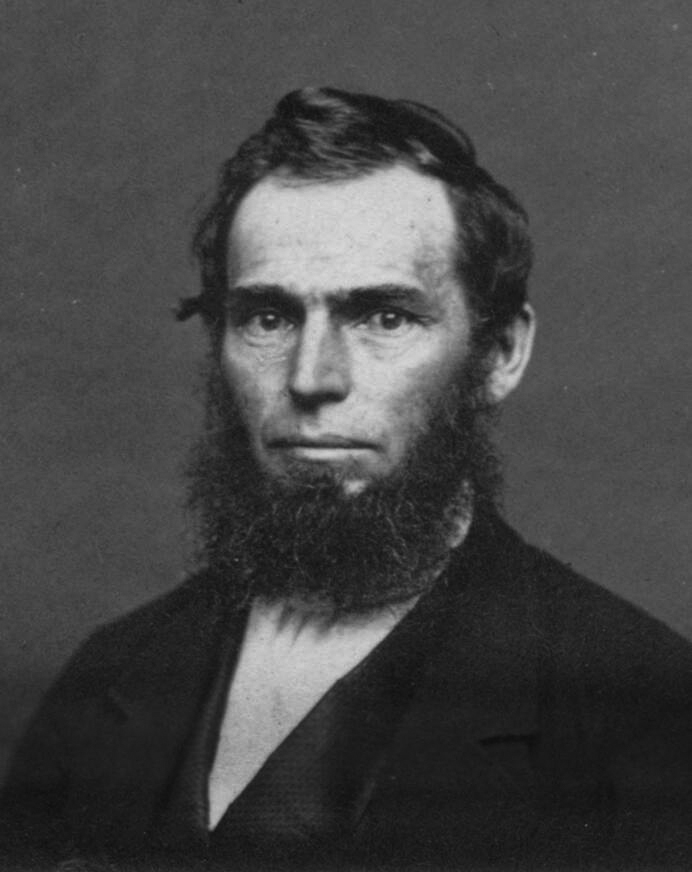
\includegraphics[width=1\linewidth]{images/j-b-frisbie.jpg}
    \caption*{John Byington Frisbie (1816-1882)}
    \label{fig:j-b-frisbie}
\end{figure}

\section*{Bog subote}

\others{Nakon što znamo i što se sjećamo Boga, održavajući Njegovu svetu Subotu, \textbf{Biblija će nas naučiti o Njegovoj ličnosti i prebivalištu}. \textbf{Čovjek je stvoren na sliku Božju, Njemu slična}. Postanak 1:26. ‘I reče Bog: Načinimo (govoreći svojemu Sinu) čovjeka na svoju sliku, nama slična.’ Poglavlje 2:7. ‘I Gospod, Bog, načini čovjeka od praha zemaljskog, i u nosnice mu udahne dah života; i čovjek postade duša živa.’ Postanak 9:6; 1 Korinćanima 11:7; Jakov 3:9. \textbf{Ono što je stvoreno na \underline{sliku i priliku Božju}, napravljeno od praha zemaljskog, nazvano je čovjekom}.}

\othersnogap{Da je upravo to pravi smisao poznato nam je iz drugih svjedočanstava koja su nam dana iz Biblije. \textbf{Isus je bio u obliku čovjeka i savršen otisak Očeve osobe}.}

\othersnogap{Filipljanima 2:6-8. \textbf{Krist Isus}: ‘koji se, premda u \textbf{obličju Božjem}, nije otimao da bude \textbf{jednak Bogu}, nego sama sebe obezvrijedi uzevši \textbf{obličje sluge} i postavši \textbf{ljudima sličan}’. 2 Korinćanima 4:4. ‘\textbf{I našavši se u obličju poput čovjeka}’, itd. Kološanima 1:15. \textbf{‘On je slika Boga nevidljivoga’}.}

\othersnogap{Hebrejima 1:3. \textbf{Sin; ‘koji je odsjaj slave i otisak bića Njegova’}. U tom smislu je Isus i mogao reći Filipu: ‘Tko je vidio mene, vidio je Oca.’ Ivan 14:9. Nekima se čini da se ovo \textbf{protivi Božjoj ličnosti, \underline{jer je on Duh, i onda kažu da je On bez tijela ili dijelova}}. Ivan 4:24. ‘\textbf{Bog je Duh}’. Hebrejima 1:7. ‘\textbf{Koji anđele svoje čini duhovima}’. \textbf{Tko će ikada tvrditi da anđeli nemaju tijela ili dijelove jer su duhovi}? \textbf{\underline{Ipak, Bog je duhovno biće koje ima tijelo i dijelove kao što možemo vidjeti iz činjenice da on ima svoje prebivalište i zato što ima tijelo i može se vidjeti}}. Izlazak 33:23. ‘Onda ću ruku svoju maknuti, pa ćeš me \textbf{vidjeti odostraga}, ali se \textbf{lice moje ne može vidjeti}’. Matej 5:8. ‘Blaženi koji su čista srca, jer \textbf{oni će Boga gledati}!’. Hebrejima 12:14. ‘Težite za mirom sa svima, i za posvećenjem, bez kojega \textbf{nitko neće vidjeti Gospodina}!’. Matej 18:10. ‘anđeli njihovi na nebesima \textbf{neprestano gledaju lice Oca mojega koji je na nebesima}.’ Matej 6:9. ‘Vi dakle molite ovako: \textbf{Oče naš koji jesi na nebesima}’, itd. Ivan 6:38. ‘Jer \textbf{siđoh s neba} ne da vršim svoju volju, nego volju onoga koji me posla’. Poglavlje 16:28. ‘\textbf{Izašao sam od Oca i došao na svijet}: Opet \textbf{ostavljam svijet i odlazim k Ocu}’.}

\othersnogap{\textbf{Ne kaže li Bog da On ispunjava prostranstvo prostora? \underline{Mi odgovaramo, Ne}}: Ps. 139:7, 8. ‘Kamo da odem \textbf{od Duha tvojega} i kamo da od \textbf{prisutnosti tvoje} pobjegnem? Ako se popnem na nebo, ti si ondje’, itd. \textbf{\underline{Bog svojim Duhom ispunjava nebo i zemlju}}, itd. \textbf{Neki miješaju Boga sa Njegovim Duhom, što čini zbunjenost}. Psalam 11:4. ‘\textbf{Gospod je u svom svetom Hramu, u nebu je prijestolje Gospodnje}: Oči njegove motre’, itd. Habakuk 2:20; Psalam 102:19. ‘Jer on gleda \textbf{s visine svetišta svojega}; \textbf{\underline{s nebesa} Gospod promatra zemlju}’. 1 Petrova 3:12. ‘Jer su oči Gospodnje nad pravednima i uši mu priklonjene molitvama njihovim’, itd. Psalam 80:1. ‘Pastiru Izraelov, čuj, ti što vodiš Josipa kao stado, ti što \textbf{sjediš među kerubima}, zasjaj’. Psalam 99:1; Izaija 37:16.}

\othersnogap{Ivan 14:2. ‘U domu Oca mojega ima mnogo stanova. Idem vam pripraviti mjesto’. Otkrivenje 21:2-5; Hebrejima 11:6. ‘jer tko Bogu pristupa, mora povjerovati da On jest’, itd. \textbf{Ovo svjedočanstvo smatramo iznimno važno u ovo vrijeme, da znamo da postoji Bog. Nema sumnje da bi, ukoliko bi nam se oči mogle otvoriti u viziji ili vidjeti onako kako anđeli vide, vidjeli bismo Boga na nebu koji sjedi na Njegovu prijestolju, i da je prisutan pred svime što postoji, koliko god ono daleko od njega bilo u Njegovom stvaranju}.}[\href{https://documents.adventistarchives.org/Periodicals/RH/RH18540307-V05-07.pdf}{Adventist Review and Sabbath Herald, 7. ožujka, 1854}, J. B. Frisbie, “The Seventh-Day Sabbath Not Abolished”, str. 50]

Ovdje vidimo isti argument i rezoniranje, da je Bog osobno duhovno Biće. Taj Bog je Bog subote. Brat Frisbie uspoređuje ovog Boga s Bogom nedjelje, koji je trinitarijanski bog.

\section*{Bog Nedjelje}

\others{Izvaditi ćemo nekoliko citata, kako bi čitatelj mogao \textbf{vidjeti široki kontrast između \underline{Boga Biblije} u svjetlosti držanja Subote, u usporedbi sa bogom tame kroz držanje nedjelje}. Katolički katekizam skraćen od strane Rt. Rev. John Duboisona, biskup iz New Yorka. Stranica 5. ‘\textbf{P: Gdje je Bog? O: Bog je svugdje prisutan}. P: Da li Bog sve vidi i sve zna? O: Da, on sve zna i vidi sve. \textbf{P. Da li Bog ima tijelo? O. \underline{Ne; Bog nema tijelo, on je čisti Duh}}. \textbf{P. Postoje li više Bogova nego jedan? O. Ne; postoji samo jedan Bog. P. Postoje li više osoba u Bogu? O. \underline{Da; u Bogu postoje tri osobe}. P. Koji su oni? O. Bog Otac, Bog Sin i Bog Sveti Duh. P. Nisu li oni tri Boga? O. Ne; Otac, Sin i Duh Sveti, su svi jedan i isti Bog}’.}

\othersnogap{Prvi članak metodističke religije, str. 8. \textbf{‘Postoji samo jedan živi i istinski Bog}, vječan, \textbf{bez tijela ili dijelova}, beskrajne moći, mudrosti i dobrote: stvoritelja i čuvara svih stvari, vidljivih i nevidljivih. \textbf{I u jedinstvu ovog Božanstva, postoje tri osobe jedne substance, moći i vječnosti; Oca, Sin i Duh Sveti}’.}

\othersnogap{U ovom članku poput katoličke doktrine \textbf{rečeno je da postoje tri osobe jedne supstance}, moći i vječnosti koje \textbf{svi zajedno čine jednog živog i istinskog Boga}, vječnog \textbf{bez tijela ili dijelova}. No u svemu tome nisu nam rekli \textbf{što se dogodilo sa Isusovim tijelom kojeg je imao nakon što je uskrsnuo, kada je otišao k Bogu koji je ‘svugdje’ ili nigdje}. Doksologija.}

\othersnogap{‘\textbf{Bog Otac, Bog Sin,’}} \\
\others{\textbf{‘Bog Duh, tri u jednom.’}} \\
\others{Ponovno} \\
\others{‘Toplina u suncu, osvježenje u povjetarcu,} \\
\others{Sjaj u zvijezdama, i cvat u drveću.} \\
\others{\textbf{Životi kroz cijeli život, proteže se u cijeloj mjeri},} \\
\others{Širi ne podijeljeno i djeluje nepotrošeno.’ - Papa.}

\othersnogap{Te su ideje dobro suglasne s onim poganskim filozofima. Jedan kaže: ‘Ta voda je načelo svih stvari i Bog je ta inteligencija kojom se sve oblikuje iz vode.’ Drugi je rekao: ‘Taj je zrak Bog, da je proizveden, da je golem i beskrajan,’ Itd. Treći, ‘To je Bog duša raspršena u svim bićima prirode’, itd. \textbf{To su neki, koji su imali ideju \underline{čistog Duha}}. Posljednja od svega, ‘Da je Bog vječna supstanca’.}

\othersnogap{Ovi izvadtci su preuzeti iz Rollin's History, sv. II, str. 597-8, objavljen od strane Harpersa. \textbf{Zar bi trebali sumnjati da je bog nedjelje došao iz istog izvora iz kojeg je došlo i čuvanje nedjelje}. ‘Nedjelja je ime koje su pogani dali prvom danu u tjednu, jer je to bio dan kada su obožavali sunce.’ - Union Bible Dictionary. \textbf{Potom je izmijenjena od strane Rimokatoličke crkve, u oblik u kojem je trenutno naučavana}.}

\othersnogap{Vrlo je prirodno pretpostaviti da kada \textbf{se Papa postavio da bude Bog u hramu Božjem}, [2 Solunjanima 2:4] da bi trebao imati dan posvećen njegovom obožavanju. To je i učinio. - Douay katekizam, str. 59. ‘P. Koji je najbolji način da se posveti nedjelja? O. Slušanjem mise, itd. Time rečeno, misa je za svećenika da se zaludi nad latinskim, pije vino i daje ljudima hostiju za jelo.’} \others{Ali Bog je posvetio svoj dan jer je počinuo na taj dan. Poseban dan za posebne svrhe. Postanak 2:3.}

\othersnogap{U danima prije moralnog pada Babilona, Bog je usmjerio umove svoje iskrene djece u njihovim molitvama na ispravan put, što god da su mislili u druga vremena, ali sada dok je um u otpadništvu molitva ne dopire do ni jednoga boga, nego samo do ljudi, ima mnogo molitava ljudima koje prepoznajemo po njihovom djelovanju i rječitosti. \textbf{Uistinu smo zahvalni našem nebeskom Ocu da je \underline{odveo naše misli od takve gluposti}, već da znamo i da se sjećamo \underline{njegovog svetog Imena} održavajući Njegov sveti Dan da bismo Ga voljeli, da bi Mu služili i dostojno \underline{Ga proslavili kroz našeg Velikog Svećenika u nebeskom Svetištu u ovom Velikom Danu Pomirenja}}.}[Ibid.][https://documents.adventistarchives.org/Periodicals/RH/RH18540307-V05-07.pdf]

Prije nego što je postao adventist sedmog dana, Frisbie je bio metodistički propovjednik i ogorčeni protivnik adventističkih vjerovanja. Godine 1853., nakon rasprave o suboti s Josephom Batesom, promijenio je svoj stav i počeo svetkovati subotu i propovijedati doktrinu adventista sedmog dana. Odrekao se nedjelje, Trojstva i prihvatio sedmi dan subote i istinu o Bogu, koju su adventisti sedmog dana naučavali u prvoj točki \emcap{Fundamentalnih Principa}.

Vide li i drugi adventistički pioniri nesklad između doktrine o Trojstvu i \emcap{ličnosti Boga} izražene u prvoj točki \emcap{Fundamentalnih Principa}?

% The Sabbath God vs. Sunday God - J. B. Frisbie

\begin{titledpoem}
    
    \stanza{
        Dva boga, dvije istine se bore, \\
        Jedan stvaran, drugi plod zablude. \\
        Jedan je Osoba s tijelom i likom, \\
        Drugi je trojstvo s čudnim oblikom.
    }

    \stanza{
        Istina o Bogu u Pismu stoji, \\
        Dok laž o trojstvu mnoge osvoji. \\
        Bog je Osoba, stvarna i živa, \\
        Ne formula što razum skriva.
    }

    \stanza{
        Na nebu sjedi naš Otac dragi, \\
        Sin Mu s desne, zastupnik blagi. \\
        Duhom svojim svuda djeluje, \\
        Ali osobno na nebu kraljuje.
    }

    \stanza{
        Subota svjedoči o Stvoritelju pravom, \\
        Koji počinu sedmoga dana sa slavom. \\
        Nedjelja pak o bogu govori, \\
        Kojeg ljudska mudrost izmisli i stvori.
    }

    \stanza{
        Bog nedjelje je "svugdje prisutan", \\
        Bez tijela, bez dijelova, trojstvom obuzdan. \\
        Iz poganskih izvora ta doktrina teče, \\
        Gdje filozofi o "čistom Duhu" rekoše.
    }

    \stanza{
        Izaberimo Boga koji počinu sedmi dan, \\
        Osobu stvarnu, ne filozofski san. \\
        Jer dan koji svetkujemo otkriva jasno, \\
        Kojem se Bogu klanjamo iskreno i glasno.
    }

\end{titledpoem}
